% !TeX root = ../libro.tex
% !TeX encoding = utf8
\chapter{Algunos métodos para resolver sistemas de ecuaciones integrales de Volterra de segunda clase}
\section{Introducción}
Los sistemas de ecuaciones integrales, lineales y no lineales, aparecen en muchas aplicaciones de ingeniería, física, química y modelos de crecimiento de poblaciones (véase en \cite{sistemas1} y \cite{sistemas2}). Las ideas generales y las características esenciales de estos sistemas se pueden aplicar en muchos ámbitos.

Una gran variedad de métodos numéricos y analíticos se usan para abordar estos sistemas, pero la mayoría encuentran dificultades en términos del gran trabajo computacional, sobre todo cuando el sistema incluye varias ecuaciones integrales. Para evitar estas dificultades que normalmente se ven en los métodos tradicionales, vamos a utilizar algunos de los métodos introducidos en el capítulo anterior, adaptándolos a este contexto más general. Los tres métodos que vamos a estudiar en este capitulo son los siguientes:
\begin{itemize}
	\item Método de descomposición de Adomian
	\item Método de la transformada de Laplace
	\item Método de las aproximaciones sucesivas
\end{itemize}

En consonancia con el estudio analítico realizado en el capítulo 2, los sistemas de ecuaciones integrales lineales de Volterra de segunda clase, vienen dados por
\begin{equation}
	\textbf{u}(x) = \textbf{f}(x) + \int_0^x \textbf{K}(x,t)\textbf{u}(t)dt, \qquad x \in [0,B].
\end{equation}
Las funciones desconocidas $\textbf{u}(x)$ que se determinarán son continuas, aparecen dentro y fuera de la integral. Los núcleos $\textbf{K}(x,t)$ y las funciones $\textbf{f}(x)$ son funciones continuas reales dadas. A continuación veremos los métodos para resolver estos sistemas.

Al igual que en la sección anterior, la información acerca de algunos de estos métodos ha sido extraída de \cite{WazWaz}.
\section{Método de descomposición de Adomian}
Como ya vimos en caso escalar, este método descompone cada solución en la suma de una serie, donde cada componente se determina de forma recursiva. Ahora, el planteamiento es totalmente análogo:
\begin{align}
	\textbf{u}_0(x) &= \textbf{f}(x),      &   \\
	\textbf{u}_{n+1}(x) &= \int_{0}^{x} \textbf{K}(x,t)\textbf{u}_n(t)dt, \qquad n \geqslant 0.         & 
\end{align}
Este método puede utilizarse en su forma estándar o combinando los términos de ruido. Además, el método de descomposición modificado se utilizará donde sea apropiado. Veamos un ejemplo para resolver un sistema de ecuaciones integrales de Volterra utilizando este método.
\begin{ejemplo}
	Partimos del siguiente sistema:
	\begin{equation}
		\left\lbrace\begin{array}{c}u(x) = x - \dfrac{1}{6}x^4 + \displaystyle \int_{0}^{x}((x-t)^2u(t) + (x-t)v(t))dt \\ v(x) = x^2 - \dfrac{1}{12}x^5 + \displaystyle \int_{0}^{x}((x-t)^3u(t) + (x-t)^2v(t))dt. \end{array}\right.
	\end{equation}
	El método nos sugiere que los términos lineales $u(x)$ y $v(x)$ se descompongan como una serie
	\begin{equation}
		u(x) = \sum_{n=0}^{\infty}u_n(x), \qquad v(x) = \sum_{n=0}^{\infty}v_n(x),
	\end{equation}
	donde $u_n(x)$ y $v_n(x)$, $n \geqslant 0$ son los términos de $u(x)$ y $v(x)$ que encontraremos de forma recursiva.
	
	Sustituyendo las series en el sistema obtenemos
	\begin{equation}
		\sum_{n=0}^{\infty}u_n(x) = x - \dfrac{1}{6}x^4 + \int_{0}^{x}((x-t)^2\sum_{n=0}^{\infty}u_n(t) + (x-t)\sum_{n=0}^{\infty}v_n(t))dt,
	\end{equation}
	\begin{equation}
		\sum_{n=0}^{\infty}v_n(x) = x^2 - \dfrac{1}{12}x^5 + \int_{0}^{x}((x-t)^3\sum_{n=0}^{\infty}u_n(t) + (x-t)^2\sum_{n=0}^{\infty}v_n(t))dt.
	\end{equation}
	
	Las primeras componentes $u_0(x)$ y $v_0(x)$ se definen como todos los términos que no están dentro de la integral, luego transformamos el sistema en un conjunto de relaciones recursivas dadas por
	\begin{align}
		u_0(x) &= x - \dfrac{1}{6}x^4,      &   \\
		u_{k+1}(x) &= \int_{0}^{x} ((x-t)^2u_k(t) + (x-t)v_k(t))dt, \qquad k \geqslant0 ,   &
	\end{align}
	y
	\begin{align}
		v_0(x) &= x^2 - \dfrac{1}{12}x^5,      &   \\
		v_{k+1}(x) &= \int_{0}^{x} ((x-t)^3u_k(t) + (x-t)^2v_k(t))dt, \qquad k \geqslant0 .   &
	\end{align}
	Si hacemos la primera iteración obtenemos
	\begin{equation}
		u_0(x) = x - \dfrac{1}{6}x^4, \qquad u_1(x) = \dfrac{1}{6}x^4 - \dfrac{1}{280}x^7,
	\end{equation}
	y
	\begin{equation}
		v_0(x) = x^2 - \dfrac{1}{12}x^5, \qquad v_1(x) = \dfrac{1}{12}x^5 - \dfrac{11}{10080}x^8.
	\end{equation}
	Es obvio que los términos de ruido $\pm \dfrac{1}{6}x^4$ aparecen entre $u_0(x)$ y $u_1(x)$. Además, los términos de ruido $\pm \dfrac{1}{12}x^5$ aparecen entre $v_0(x)$ y $v_1(x)$. Si cancelamos estos términos de ruido en $u_0(x)$ y $v_0(x)$, el resto de términos restantes nos dan la solución exacta
	\begin{equation}
		(u(x), v(x)) = (x,x^2).
	\end{equation}
\end{ejemplo}

\section{Método de la transformada de Laplace}
Aunque ya hemos explicado este método en profundidad en el capítulo anterior en caso escalar, vamos a describir cómo sería para sistemas, y posteriormente mostraremos un ejemplo en el que veremos cómo se aplica a un sistema de ecuaciones integrales de Volterra.

Partimos de nuestro sistema
\begin{equation}
	\textbf{u}(x) = \textbf{f}(x) + \int_0^x \textbf{K}(x,t)\textbf{u}(t)dt, \qquad x \in [0,B].
\end{equation}
Tomando la transformada de Laplace de ambos lados tenemos
\begin{equation}
	\textbf{U}(s) =\textbf{F}(s) + \mathcal{\textbf{K}}(s)\textbf{U}(s),
\end{equation}
donde
\begin{equation}
	\textbf{U}(s) = \mathcal{L}\{\textbf{u}(x)\}, \qquad \mathcal{\textbf{K}}(s) = \mathcal{L}\{\textbf{K}(x)\}, \qquad \textbf{F}(s) = \mathcal{L}\{\textbf{f}(x)\}.
\end{equation}
Resolviendo la ecuación para $\textbf{U}(s)$ obtenemos
\begin{equation}
	\textbf{U}(s) = \dfrac{\textbf{F}(s)}{1- \mathcal{\textbf{K}}(s)}, \qquad  \mathcal{\textbf{K}}(s) \neq 1.
\end{equation}
La solución $\textbf{u}(x)$ se obtiene tomando la inversa de la transformada de Laplace en la ecuación anterior donde obtenemos:
\begin{equation}
	\textbf{u}(x) = \mathcal{L}^{-1}\{\dfrac{\textbf{F}(s)}{1- \mathcal{\textbf{K}}(s)}\}.
\end{equation}
\begin{ejemplo}
	Sea el sistema
	\begin{equation}
		\left\lbrace\begin{array}{c}u(x) = 1 - x^2 + x^3 + \displaystyle \int_{0}^{x}((x-t)u(t) + (x-t)v(t))dt \\ v(x) = 1 - x^3 - \dfrac{1}{10}x^5 + \displaystyle \int_{0}^{x}((x-t)u(t) - (x-t)v(t))dt. \end{array}\right.
	\end{equation}
	Es importante darse cuenta que ambos núcleos son iguales, es decir, $K_1(x-t) = K_2(x-t) = x-t$. Tomando la transformada de Laplace en ambos lados de cada ecuación obtenemos
	\begin{equation}
		U(s) = \mathcal{L}\{u(x)\} = \mathcal{L}\{1 - x^2 + x^3\} + \mathcal{L}\{(x-t)\ast u(x) + (x-t) \ast v(x)\},
	\end{equation}
	\begin{equation}
		V(s) = \mathcal{L}\{v(x)\} = \mathcal{L}\{1 - x^3 - \dfrac{1}{10}x^5\} + 	\mathcal{L}\{(x-t)\ast u(x) - (x-t) \ast v(x)\}.
	\end{equation}
	Esto al mismo tiempo nos da
	\begin{equation}
		U(s) = \dfrac{1}{s} - \dfrac{2}{s^3} + \dfrac{6}{s^4} + \dfrac{1}{s^2}U(s) + \dfrac{1}{s^2}V(s),
	\end{equation}
	\begin{equation}
		V(s) = \dfrac{1}{s} - \dfrac{6}{s^4} - \dfrac{12}{s^6} + \dfrac{1}{s^2}U(s) 	- \dfrac{1}{s^2}V(s),
	\end{equation}
	Reorganizando un poco el sistema obtenemos
	\begin{equation}
		(1-\dfrac{1}{s^2})U(s) - \dfrac{1}{s^2}V(s) = \dfrac{1}{s} - \dfrac{2}{s^3} + \dfrac{6}{s^4},
	\end{equation}
	\begin{equation}
		(1+\dfrac{1}{s^2})V(s) - \dfrac{1}{s^2}U(s) = \dfrac{1}{s} - \dfrac{6}{s^4}	- \dfrac{12}{s^6}.
	\end{equation}
	Resolviendo el sistema para $U(s)$ y $V(s)$ tenemos como resultado
	\begin{equation}
		U(s) = \dfrac{1}{s} + \dfrac{3!}{s^4},
	\end{equation}
	\begin{equation}
		V(s) = \dfrac{1}{s} - \dfrac{3!}{s^4}.
	\end{equation}
	Tomando la inversa de la transformada de Laplace en ambos lados de cada ecuación, la solución exacta viene dada por
	\begin{equation}
		(u(x),v(x)) = (1 + x^3, 1 - x^3).
	\end{equation}
\end{ejemplo}

\section{Método de aproximaciones sucesivas}
El método de aproximaciones sucesivas también se puede aplicar a sistemas de ecuaciones integrales de Volterra en el caso vectorial. Cuando tenemos un sistema de ecuaciones integrales de Volterra en forma vectorial, el procedimiento es similar al caso escalar, pero trabajaremos con vectores en lugar de con funciones escalares, es decir, tenemos que
\begin{equation}
	\textbf{u}(x) = \textbf{f}(x) + \int_0^x \textbf{K}(x,t)\textbf{u}(t)dt
\end{equation}
donde $\textbf{u}(x)$ es un vector de funciones que deseas encontrar, $\textbf{f}(x)$ es un vector de funciones conocidas, y $\textbf{K}(x,t)$ es la matriz de funciones núcleo, todos ellos continuos. Además, necesitaremos una función vectorial con las aproximaciones iniciales de cada ecuación, que denotaremos como $\textbf{u}_0$. Veamos un ejemplo:
\begin{ejemplo}
	Consideramos el siguiente sistema:
	\[ \begin{dcases}
		y(x) = 1 + \displaystyle \int_0^x (\dfrac{1}{8}y(t)-\dfrac{1}{6}v(t))dt \\
		v(x) = 3+ \displaystyle \int_0^x (\dfrac{1}{7}y(t)-\dfrac{1}{8}v(t))dt \;
	\end{dcases} \]%
	donde tenemos los siguientes vectores:
	\begin{equation}
		\textbf{u}(x) = \begin{pmatrix}	y(x) \\ v(x)	\end{pmatrix}, \qquad \textbf{f}(x) = \begin{pmatrix}	1 \\ 3	\end{pmatrix}, \qquad \textbf{K}(x,t) = \begin{pmatrix}[2]	\dfrac{1}{8} & -\dfrac{1}{6} \\ \dfrac{ 1}{7} & -\dfrac{1}{8}	\end{pmatrix},
	\end{equation}
	Además tenemos el vector de aproximaciones iniciales para ambas ecuaciones:
	\begin{equation}
		\textbf{u}_0 = \begin{pmatrix}	0 \\ 1	\end{pmatrix}.
	\end{equation}
	Por tanto la fórmula iterativa que vamos a utilizar para calcular las aproximaciones sucesivas es
	\begin{equation}
		\textbf{u}_{n+1}(x) = \textbf{f}(x) + \int_0^x \textbf{K}(x,t)\textbf{u}_n(t)dt, \qquad n \geqslant 0.
	\end{equation}
	Sustituyendo $\textbf{u}_0$ obtenemos:
	\begin{equation}
		\textbf{u}_{1}(x) = \textbf{f}(x) + \int_0^x \textbf{K}(x,t)\textbf{u}_0(t)dt = \begin{pmatrix}[2]	1-\dfrac{t}{6} \\ 3-\dfrac{t}{8}	\end{pmatrix}
	\end{equation}
	\begin{equation}
		\textbf{u}_{2}(x) = \textbf{f}(x) + \int_0^x \textbf{K}(x,t)\textbf{u}_1(t)dt = \begin{pmatrix}[2]	1-\dfrac{3t}{8} \\ -\dfrac{11t^2}{1344}-\dfrac{13t}{56}+3	\end{pmatrix}
	\end{equation}
	Una solución más aproximada con la quinta iteración sería
	\begin{equation}
		\textbf{u}_{5}(x) = \begin{pmatrix}[2.2]	-\dfrac{121t^5}{10838016}+\dfrac{121t^4}{1806336}+\dfrac{11t^3}{3584}-\dfrac{11t^2}{1344}-\dfrac{3t}{8}+1 \\ -\dfrac{121t^5}{14450688}+\dfrac{121t^4}{602112}+\dfrac{143t^3}{75264}-\dfrac{11t^2}{448}-\dfrac{13t}{56}+3	\end{pmatrix}.
	\end{equation}
	Comparamos en la \autoref{fig:sol43} la aproximación con la solución y observamos que la aproximación ya es aceptable con la quinta iteración.
	\begin{figure}[h!]
		\centering
		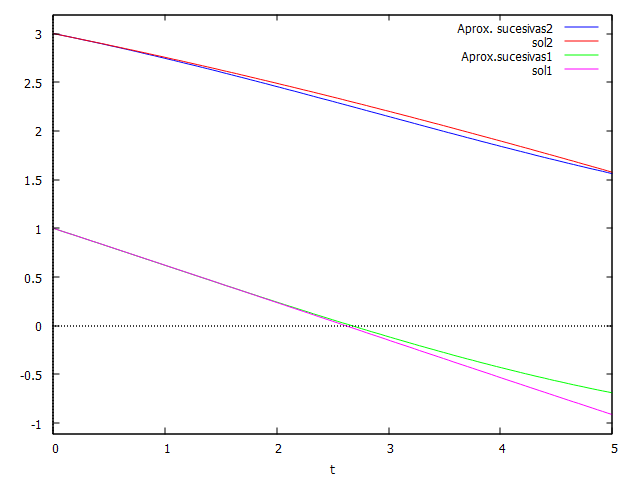
\includegraphics[width=0.8\textwidth]{comp_sol_ej43}
		\caption{Solución exacta y con aproximaciones sucesivas}
		\label{fig:sol43}
	\end{figure}
\end{ejemplo}
\begin{observacion}
	Todos los resultados de convergencia y error que vimos en el capítulo 2 para el caso escalar y que aplicamos en este método, se utilizan de forma análoga en el caso vectorial.
\end{observacion}


\endinput
%------------------------------------------------------------------------------------
% FIN DEL CAPÍTULO. 
%------------------------------------------------------------------------------------